\documentclass[12pt, titlepage]{article}

\usepackage{fullpage}
\usepackage[round]{natbib}
\usepackage{multirow}
\usepackage{booktabs}
\usepackage{tabularx}
\usepackage{graphicx}
\usepackage{float}
\usepackage{hyperref}
\hypersetup{
    colorlinks,
    citecolor=blue,
    filecolor=black,
    linkcolor=red,
    urlcolor=blue
}

%%% Comments

\usepackage{color}

\newif\ifcomments\commentstrue %displays comments
%\newif\ifcomments\commentsfalse %so that comments do not display

\ifcomments
\newcommand{\authornote}[3]{\textcolor{#1}{[#3 ---#2]}}
\newcommand{\todo}[1]{\textcolor{red}{[TODO: #1]}}
\else
\newcommand{\authornote}[3]{}
\newcommand{\todo}[1]{}
\fi

\newcommand{\wss}[1]{\authornote{blue}{SS}{#1}} 
\newcommand{\plt}[1]{\authornote{magenta}{TPLT}{#1}} %For explanation of the template
\newcommand{\an}[1]{\authornote{cyan}{Author}{#1}}

%%% Common Parts

\newcommand{\progname}{ProgName} % PUT YOUR PROGRAM NAME HERE
\newcommand{\authname}{Team \#, Team Name
\\ Student 1 name
\\ Student 2 name
\\ Student 3 name
\\ Student 4 name} % AUTHOR NAMES                  

\usepackage{hyperref}
    \hypersetup{colorlinks=true, linkcolor=blue, citecolor=blue, filecolor=blue,
                urlcolor=blue, unicode=false}
    \urlstyle{same}
                                

\newcounter{acnum}
\newcommand{\actheacnum}{AC\theacnum}
\newcommand{\acref}[1]{AC\ref{#1}}

\newcounter{ucnum}
\newcommand{\uctheucnum}{UC\theucnum}
\newcommand{\uref}[1]{UC\ref{#1}}

\newcounter{mnum}
\newcommand{\mthemnum}{M\themnum}
\newcommand{\mref}[1]{M\ref{#1}}

\begin{document}

\title{Module Guide for \progname{Physics Game Based on Angry Birds}} 
\author{Al Jubair Hossain}
\date{\today}

\maketitle

\pagenumbering{roman}

\section{Revision History}

\begin{tabularx}{\textwidth}{p{3cm}p{2cm}X}
\toprule {\bf Date} & {\bf Version} & {\bf Notes}\\
\midrule
March 4, 2024 & 1 & Changed section (Hyperlink)\\
March 12, 2024 & 2 & Changed section (7)\\
\bottomrule
\end{tabularx}

\newpage

%\section{Reference Material}

%This section records information for easy reference.

%\subsection{Abbreviations and Acronyms}

%\renewcommand{\arraystretch}{1.2}
%\begin{tabular}{l l} 
 % \toprule		
%  \textbf{symbol} & \textbf{description}\\
 % \midrule 
 % AC & Anticipated Change\\
 % DAG & Directed Acyclic Graph \\
%  M & Module \\
 % MG & Module Guide \\
%  OS & Operating System \\
 % R & Requirement\\
%  SC & Scientific Computing \\
%  SRS & Software Requirements Specification\\
%  \progname & Explanation of program name\\
 % UC & Unlikely Change \\
 % \wss{etc.} & \wss{...}\\
 % \bottomrule
%\end{tabular}\\

\newpage

\tableofcontents

\listoftables

\listoffigures

\newpage

\pagenumbering{arabic}

\section{Introduction}
\subsection{Purpose of the Module Guide}
The purpose of this Module Guide is to provide an in-depth understanding of the software modules that constitute the Sample Physics-Based Game. It outlines the individual modules' functionalities, dependencies, interfaces, and relationships, offering insights into the game's architecture and design. The guide is intended for developers, architects, and other stakeholders involved in the development, testing, and maintenance of the game.
\subsection{Scope}
This Module Guide focuses on documenting the specifics of each software module within the Sample Physics-Based Game. It covers modules related to physics simulation, game elements, user interaction, graphics, and sound. The scope includes detailed descriptions of each module's purpose, functionalities, and interactions with other modules.

\section{Game Overview}
\subsection{Game Description}
The game is a physics-based gaming application designed to provide players with an engaging and challenging experience. Players interact with the game environment by manipulating objects, analyzing trajectories, and applying physics principles. The central focus is on realistic collision dynamics, gravitational forces, and other physical phenomena..

\subsection{Physics Simulation}
The heart of the game lies in its physics simulation, where realistic collision interactions between a projectile and targets/obstacles are implemented. Gravity influences the trajectory and motion of the projectile, adding an authentic touch to in-game dynamics. Additionally, the game introduces the option to consider additional forces, such as wind, for heightened complexity. Visual feedback for collisions, including deformation or destruction of targets, enhances the overall gaming experience.
\subsection{Game Architecture}
\subsubsection{High-Level Components}
\begin{itemize}
    \item \textbf{User Input:} Receives and interprets input from players, allowing them to interact with the game.
    \item \textbf{Launch Controls:} Manages the parameters for launching the projectile, providing options for adjusting launch angle, force, and other relevant parameters.
    \item \textbf{Projectile Logic:} Governs the behavior and properties of the projectile, including its initial position, velocity, and mass.
    \item \textbf{Physics Engine: } Orchestrates the physics simulation, encompassing collision detection, gravity simulation, and the consideration of additional forces.
    \item \textbf{Graphics Module:} Enhances the visual appeal of the game, handling the rendering of objects and visual feedback for collisions.
    \item \textbf{Sound Effects:} Complements the gameplay experience by implementing auditory elements tied to in-game events.
\end{itemize}

\subsubsection{Interactions between Components}
\begin{itemize}
    \item User Input influences Launch Controls, allowing players to control the launch parameters.
    \item Launch Controls communicate with Projectile Logic to define the projectile's characteristics.
    \item Physics Engine interacts with Projectile Logic for realistic collision interactions, gravity simulation, and handling additional forces.
    \item Graphics Module receives information from Physics Engine to render visual elements, providing feedback for collisions.
    \item Sound Effects are triggered based on events detected by the Physics Engine, enriching the auditory aspect of the game.
\end{itemize}
\subsection{Dependencies on External Systems}
The game is dependent on external systems, potentially involving compatibility with graphics libraries or leveraging external physics engines. Understanding and managing these dependencies are crucial for ensuring a seamless and optimized gaming experience.

\section{Module Descriptions}
\subsection{Module}
\subsubsection{Purpose}
The Bird module represents the player-controlled projectile in the game, defining its initial properties and behavior
\subsubsection{Functionality}
\begin{itemize}
    \item Initialization of the bird's position, velocity, and mass.
    \item Handling user-triggered launches and applying realistic physics for projectile motion.
    \item Collision detection with game elements.
\end{itemize}

\subsubsection{Dependencies}
\begin{itemize}
\item Dependent on the game physics module for realistic collision interactions.
\item Interfaces with the user interaction module to receive launch commands.
\end{itemize}

\subsubsection{Interfaces}
\begin{itemize}
    \item Input Interface(s):
    \item User interaction module for launch commands.
    \item Output Interface(s):
    \item Interfaces with the game physics module for collision information.
\end{itemize}

\subsubsection{Module Relationships}
\begin{itemize}
    \item Dependencies:\\
    •	Relies on the game physics module for collision interactions.
    \item Dependents: \\
    •	Other modules may depend on collision information from the Bird module.
\end{itemize}

\section{Data Design}
\subsection{Physics Data Structures}
\subsubsection{Purpose}
	This section outlines the data structures employed for managing physics-related information within the game. The design focuses on representing projectile properties, collision data, and other parameters crucial for realistic physics simulation.
\subsubsection{ Data Structures}
\begin{enumerate}
    \item Projectile Properties:
    \begin{itemize}
        \item Definition: Stores information such as position, velocity, and mass of the projectile.
        \item Usage: Utilized by the Physics Engine to calculate and update the projectile's motion.
    \end{itemize}
    \item Collision Data:
        \begin{itemize}
            \item Definition: Captures data related to collisions, including collision points and impact forces.
            \item Usage: Enables accurate collision response and provides information for visual and auditory feedback.
        \end{itemize}
\end{enumerate}

\subsection{Game State Management}
\subsubsection{Purpose}
This section delves into the design of the game state management system, responsible for capturing and maintaining the overall state of the game. It encompasses information related to scores, levels, and the current status of game elements.
\subsubsection{Data Structures}
\begin{enumerate}
    \item Game State
        \begin{itemize}
            \item Definition: Represents the overall state of the game, including scores, level progression, and other relevant parameters.
            \item Usage: Provides a centralized repository for managing and updating the current state of the game.
        \end{itemize}
\end{enumerate}

\subsection{Input Data Handling}
\subsubsection{Purpose}
	Detailing the data structures and mechanisms employed for handling user input. This includes capturing and interpreting input from players to control game elements.
\subsubsection{Data Structures}
\textbf{User Input Data:}
    \begin{itemize}
        \item Definition: Stores information received from user inputs, such as mouse clicks or touch events.
        \item Usage: Feeds input data to the User Interface and Launch Controls for further processing.
    \end{itemize}

\subsection{Data Flow}
\subsubsection{Purpose}
Explaining the flow of data within the game, illustrating how information moves between different components and modules

\subsubsection{Data Flow Pathways}
\begin{enumerate}
    \item \textbf{User Input to Launch Controls:}
    \begin{itemize}
        \item  Flow: User Input data is transmitted to Launch Controls for interpreting player actions.
    \end{itemize}
    \item \textbf{Launch Controls to Projectile Logic:}
    \begin{itemize}
        \item Flow: Launch parameters are communicated to Projectile Logic for configuring the projectile's initial properties.
    \end{itemize}
    \item \textbf{Physics Engine to Graphics Module:}
    \begin{itemize}
        \item Flow: Information regarding collisions and physics simulations is conveyed to the Graphics Module for rendering visual feedback.
    \end{itemize}
    \item \textbf{Physics Engine to Sound Effects:}
    \begin{itemize}
        \item Flow: Events detected by the Physics Engine trigger Sound Effects for auditory feedback.
    \end{itemize}
   
\end{enumerate}

\section{Component Design}
\subsection{Component 1: Physics Simulation Component}
\subsubsection{Purpose}
The Physics Simulation Component is designed to handle the realistic physics interactions within the game. It governs the motion of projectiles, detects collisions, and manages gravitational influences to create an authentic gaming experience.

\subsubsection{Functionality}
\begin{enumerate}
    \item Projectile Motion:
    \begin{itemize}
        \item Utilizes physics equations to calculate and update the motion of projectiles based on their initial conditions.
    \end{itemize}
\item Collision Detection
    \begin{itemize}
        \item Implements algorithms for detecting collisions between projectiles and targets/obstacles within the game environment.
    \end{itemize}
 \item Gravity Simulation:
    \begin{itemize}
        \item Applies gravitational forces to influence the trajectory and motion of projectiles
    \end{itemize}
\end{enumerate}

\subsubsection{Dependencies}
    \begin{itemize}
        \item Physics Data Structures: Relies on data structures to access and manipulate physics-related information, including projectile properties and collision data.
    \end{itemize}

\subsubsection{Interfaces}
    \begin{enumerate}
        \item \textbf{Input Interface:}
            \begin{itemize}
                \item Receives input from the Launch Controls and Projectile Logic modules for initializing projectile properties.
            \end{itemize}
        \item \textbf{Output Interface:}
            \begin{itemize}
                \item Communicates collision data to the Graphics Module for rendering visual feedback.
            \end{itemize}
    \end{enumerate}

\subsubsection{Interaction with Modules}
\begin{itemize}
    \item Launch Controls:
        \begin{itemize}
            \item Receives launch parameters to set the initial conditions for projectiles.
        \end{itemize}
    \item Projectile Logic:
        \begin{itemize}
            \item Collaborates to integrate realistic physics calculations into the game's projectile behavior.
        \end{itemize}
\end{itemize}

\subsection{Component 2: User Input Component}
\subsubsection{Purpose}
The User Input Component serves as the interface between players and the game, capturing and interpreting user inputs to control various aspects of gameplay.

\subsubsection{Functionality}
\begin{enumerate}
    \item Input Capture:
    \begin{itemize}
        \item Captures user inputs, including mouse clicks or touch events.
    \end{itemize}
    \item Input Interpretation:
        \begin{itemize}
            \item Translates captured inputs into meaningful commands for the game.
        \end{itemize}
\end{enumerate}

\subsubsection{Dependencies}
None identified. The User Input Component operates independently of other components.

\subsubsection{Interfaces}
\begin{enumerate}
    \item Output Interface:
        \begin{itemize}
            \item Transmits interpreted user inputs to the Launch Controls for further processing.
        \end{itemize}
\end{enumerate}

\subsubsection{Interaction with Modules}
\begin{enumerate}
    \item Launch Controls:
        \begin{itemize}
            \item Provides interpreted user inputs to influence launch parameters and initiate projectile launches.
        \end{itemize}
\end{enumerate}

\section{Quality Attributes}
\subsection{Physics Simulation Accuracy}
\subsubsection{Definition}
Physics Simulation Accuracy evaluates the precision of in-game physics calculations, ensuring the faithful representation of real-world principles. It demands a meticulous implementation of equations such as the equations of motion $s=ut+\frac{1}{2}at^2$ 
for projectile motion and Newton's law of universal gravitation $F=Gm_1m_2/r^2$ for gravitational interactions.

\subsubsection{Evaluation Criteria}
\begin{itemize}
    \item Accurate Projectile Motion Equations:
    \begin{itemize}
        \item Implementing projectile motion equations with precision to model the realistic trajectory of objects in the game.
    \end{itemize}
    \item Faithful Application of Newton's Law of Gravitation:
        \begin{itemize}
            \item Ensuring that gravitational interactions closely follow Newton's law, contributing to the authenticity of in-game physics.
        \end{itemize}
\end{itemize}

\subsection{Gameplay Responsiveness}
\subsubsection{Definition}
Gameplay Responsiveness measures the system's agility in responding to player inputs using principles like kinematics equations ($s=ut+\frac{1}{2}at^2$). It emphasizes minimizing the time between a player's action and the corresponding in-game reaction.

\subsubsection{Evaluation Criteria}
\begin{itemize}
    \item Low Input-to-Action Latency with Kinematics:
        \begin{itemize}
            \item Minimizing the time delay between a player's input (e.g., launching a projectile) and the resulting in-game action, applying kinematics equations.
        \end{itemize}
      \item Consistent and High Frame Rate for Responsive Controls:
        \begin{itemize}
            \item Maintaining a high and consistent frame rate to ensure fluid animations and responsiveness, drawing from principles of dynamics ($F = ma$).
        \end{itemize}
	
\end{itemize}

\subsection{Scalability}
    \subsubsection{Definition}
Scalability assesses the game's capability to handle increasing complexity and additional features, considering principles like force and acceleration $(F = ma)$. It ensures optimal performance under varied scenarios.
\subsubsection{Evaluation Criteria}
\begin{itemize}
    \item Optimal Performance under Increased Load using Newton's Second Law:
       \begin{itemize}
           \item Ensuring the game performs optimally even with a larger number of projectiles, targets, or complex scenarios, applying Newton's second law of motion.
       \end{itemize} 
       \item Adaptability to New Features applying Force Equations:
        \begin{itemize}
            \item Evaluating how easily new features or challenges can be integrated, incorporating force equations $(F = \Delta p/\Delta t$.)
        \end{itemize}
\end{itemize}

\subsection{Maintainability}
\subsubsection{Definition}
Maintainability evaluates the ease of updating, enhancing, and debugging the game over its lifecycle. It emphasizes modular design and comprehensive documentation, akin to principles of work and energy (W = ΔKE).
\subsubsection{Evaluation Criteria}

\begin{itemize}
    \item \textbf{Modular Design for Work-Energy Principles:}
       \begin{itemize}
  \item Utilizing modular design principles and organized code for ease of updates and modifications, inspired by principles of work and energy.
        \end{itemize}

    \item \textbf{Comprehensive Documentation for Clear Understanding:}
        \begin{itemize}
            \item Providing thorough documentation for clarity and understanding, reflecting the documentation practices in physics principles.
        \end{itemize}
\end{itemize}

\subsection{Usability}
\subsubsection{Definition}
	Usability assesses how easily players can interact with and enjoy the game. It considers intuitive controls and a clear user interface, applying principles of kinematics for control design and information visualization.
\subsubsection{Evaluation Criteria}
    \begin{itemize}
        \item Intuitive Controls with Kinematics Design:
            \begin{itemize}
                \item Ensuring controls are easy to learn and intuitive, leveraging kinematics equations to design control mechanisms.
            \end{itemize}
            \item Clear and Informative User Interface applying Information Visualization:
                \begin{itemize}
                    \item Providing a user interface that offers clear feedback and information, applying principles of information visualization for enhanced user understanding.
                \end{itemize}
    \end{itemize}

\section{Physic equation Mockup}



\begin{figure}[H]
\centering
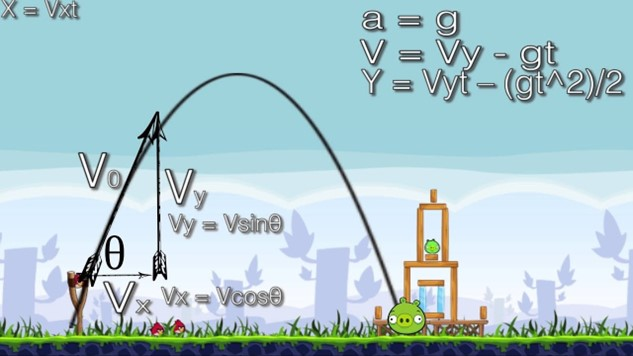
\includegraphics[width=0.5\textwidth]{fig1.jpg}
\caption{This image combines elements from 'Angry Birds' with physics equations to explain projectile motion, showing velocity components and trajectory formulas.}
\label{Fig:fig1}
\end{figure}


This image \ref{Fig:fig2} appears to be a screenshot from a video playback of a game-based learning module or educational software. It displays a projectile motion scenario within a game setting. The vectors illustrate the physics concepts of initial velocity ($v_i$) and final velocity ($v_f$), with the dotted line indicating the trajectory of the launched object. The change in velocity $\delta(v)$ is represented by an arrow pointing upwards from the final to the initial velocity, demonstrating the change in the object's speed and direction as it moves. This educational tool seems designed to help users understand the principles of kinematics by visualizing the changes in an object's velocity during projectile motion. The high score and current score are displayed in the top right, implying a gamified learning experience.

\begin{figure}[H]
\centering
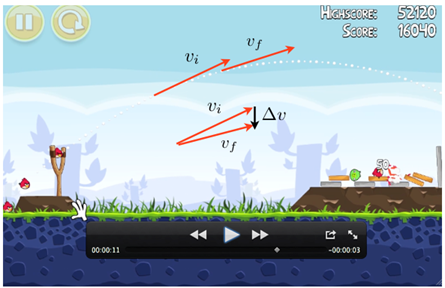
\includegraphics[width=0.55\textwidth]{fig2.png}
\caption{The image depicts a screenshot from 'Angry Birds' annotated with vectors to show initial velocity $v_i$, final velocity $v_f$, and the change in velocity $\Delta(V)$, demonstrating concepts of motion in physics.}
\label{Fig:fig2}
\end{figure}

The image \ref{Fig:fig3} appears to be a playful educational overlay on a screenshot from a game, illustrating various principles of physics in the context of projectile motion. It includes equations and notations for energy (kinetic and potential), velocity (initial and final), acceleration due to gravity, angles, and trajectory paths. Notably:
\\

$0=\frac{1}{2} m v^2+m g \Delta y$ - An energy conservation equation where kinetic energy plus potential energy equals zero, suggesting the highest point of the trajectory where velocity is zero.\\
$v=\sqrt{2 g a y}$ - An equation relating velocity to the acceleration due to gravity and the height of the projectile. \\

$a=9.8 \mathrm{~m} / \mathrm{s}^2$ - The acceleration due to Earth's gravity. \\
$v_x=\sqrt{(k x)^2 / m}-2 g s \sin \theta$ - An equation for horizontal velocity taking into account spring constant, mass, gravity, and angle of launch. \\
$\tan \theta=v_y / v_x$ and $\theta=\tan ^{-1}\left(v_y / v_x\right)$ - Equations for calculating the launch angle using the tangential function with vertical and horizontal velocity components. \\
$y_e=h+s \sin \theta$ - A trigonometric equation for the vertical displacement. \\

The image also includes a free body diagram for the angles of projection and force vectors at the launch point, and it visually depicts the projectile's parabolic path through the game's environment. The game's high score is visible, implying that understanding these physics concepts could be used to strategize and improve gameplay performance.

\begin{figure}[H]
\centering
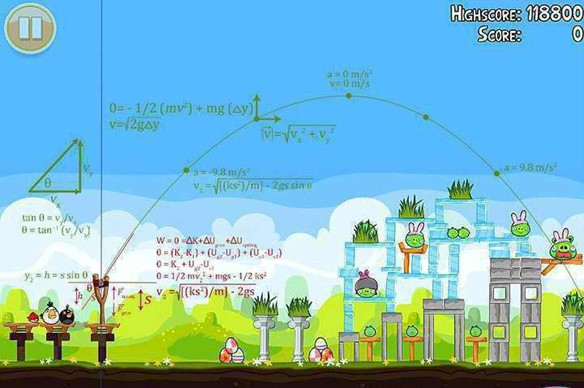
\includegraphics[width=0.7\textwidth]{fig3.jpg}
\caption{Use hierarchy among modules}
\label{Fig:fig3}
\end{figure}

\begin{figure}[H]
\centering
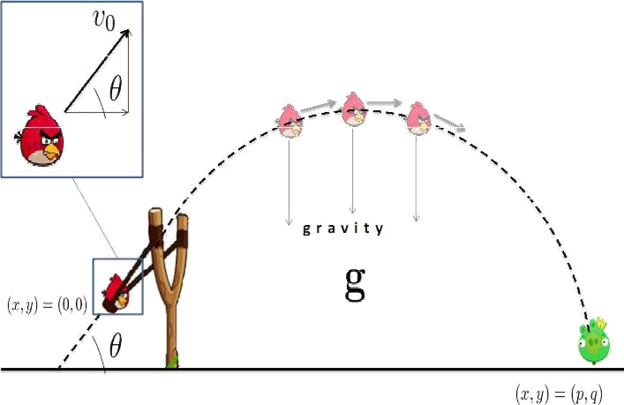
\includegraphics[width=0.7\textwidth]{fig4.png}
\caption{The image demonstrates a physics problem using 'Angry Birds', showing a bird being launched from a slingshot at an angle $\theta$ with initial velocity $v_o$, aiming to hit targets A and B placed at different heights and distances.}
\label{Fig:fig4}
\end{figure}

This image \ref{Fig:fig5} is a simple graphical representation of projectile motion at different angles. It illustrates three separate trajectories for an object launched from a catapult at angles of 70°, 45°, and 20° above the horizontal. The height and range of each trajectory vary with the angle of launch. The 45° angle is commonly known to give the maximum range under ideal conditions without air resistance. Each trajectory is marked with points that likely represent equal time intervals, demonstrating how the angle affects both the time of flight and the horizontal distance traveled by the projectile. This kind of diagram is typically used in physics education to teach the principles of projectile motion.

\begin{figure}[H]
\centering
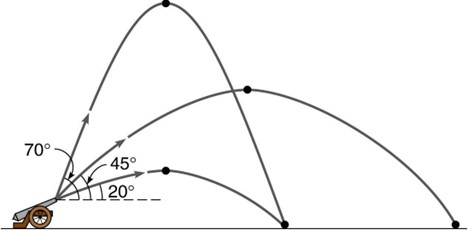
\includegraphics[width=0.7\textwidth]{fig5.jpg}
\caption{The image shows trajectories of projectiles launched at different angles -20°, 45°, and 70° to illustrate the range of motion in physics, with the 45° angle likely providing the greatest range.}
\label{Fig:fig5}
\end{figure}



\end{document}